%% ----------------------------------------------------------------
%% SETTINGS
%% ----------------------------------------------------------------
\documentclass[../et.tex]{subfiles}

%% ----------------------------------------------------------------
%% BEGIN
%% ----------------------------------------------------------------
\begin{document}

%% ----------------------------------------------------------------
%% DOCUMENT
%% ----------------------------------------------------------------
El diseño de firmware consiste en la creación del proceso de decisión que se lleva a cabo en el microcontrolador. Este luego ha sido programado en lenguaje C, sin utilizar ningún sistema operativo en tiempo real (RTOS) y con la ayuda del Advanced Software Framework (ASF) de Atmel, que provee una capa de abstracción de hardware, facilitando así el uso de los periféricos.

Esta sección responde a los requerimientos RF01 y RF02.

%% ----------------------------------------------------------------
\subsection{Estructura general}
%% ----------------------------------------------------------------
El código se ha dividido en módulos llamados \textit{apps}. Cada uno de ellos cuenta con un \textit{api} que será el encargado de comunicarse con la interfaz de comunicaciones, así permitiendo tener una capa de abstracción entre ambos. Por último, esta interfaz de comunicaciones además de contar con su propio \textit{api} para comunicarse con los módulos, provee también la estructura necesaria para poder comunicarse con la PC, ya sea vía UART o USB.

Esta estructura se puede ver en la \autoref{fig:firmware-general}.

    \begin{figure}[!htbp]
        \centering
        \includegraphics[scale=0.23]{diagrams/firmware-general.png}
        \caption{Estructura general de los módulos en el microcontrolador}
        \label{fig:firmware-general}
    \end{figure}


Las distintas partes que componen el firmware son:
  \begin{itemize}
      \item Módulo de comunicaciones
      \item Módulo de control
      \item Módulo de adquisición y procesamiento de señales
      \item Módulo de generación de corriente
  \end{itemize}

De estos se explicarán algunos que vale la pena resaltar.

%% ----------------------------------------------------------------
%% SUB-SUB-SECCIÓN
%% ----------------------------------------------------------------
\subsection{Módulo de comunicaciones}
%% ----------------------------------------------------------------
Este módulo es el encargado de enviar y recibir comunicaciones entre el microcontrolador y la PC. La característica de diseño del mismo es que su función sea solamente receptiva: esto es, el microcontrolador nunca iniciará una comunicación por si cuenta, sólo responderá. Se ahorra así la implementación de un esquema de acceso al medio.

Se diseñó entonces un sencillo protocolo de comunicaciones mostrado a continuación:

\begin{table}[!htbp]
    \centering
    \begin{tabular}{c|c|c|c|c|c|c|c}
    Inicio & Proyecto & Fuente & Destino & Longitud & Datos & $...$ & CRC
    \end{tabular}
\end{table}

Cada bloque representa un byte, excepto el CRC (código de corrección de errores) que es de dos bytes. Tanto el byte de inicio, como el de proyecto, fuente y destino, son configurables. La longitud representa la cantidad de datos enviados y el CRC se genera y verifica solo.

Se permite realizar la comunicación de dos formas. La primera es utilizando la UART y conectando la PC a través de un convertidor. La segunda y más cómoda es utilizar el puerto USB. Una vez conectado, el mismo funcionará generando un puerto COM virtual, a través del cual se puede enviar y recibir información.

%% ----------------------------------------------------------------
\subsection{Módulo de control}
%% ----------------------------------------------------------------
Este módulo es la implementación del mecanismo de control a partir del cual se genera una corriente precisa. Esto se logra realimentándola y comparando la medición con un valor de referencia, obteniendo así un error que se desea minimizar.

\paragraph{Estrategia de control}
Si bien hay varias estrategias de control para sistemas con señales de referencia alternas, se decidió utilizar un esquema de control repetitivo (RC) tal como está descripto en \cite{control-lic}.

La ventaja del controlador repetitivo respecto al controlador resonante, otra opción explorada, es que este último introduce polos en $s = \pm j\omega_0$, debiendo introducir tantos controladores como frecuencias se quieran controlar. En cambio, el RC, al estar basado en el principio del modelo interno, introduce polos en $s = \pm jn\omega_0$, de manera de permitir seguir tanto la señal fundamental como sus armónicos, obteniendo así mejor performance.

\paragraph{Diagrama en bloques}
Es necesario entonces, definir la estructura del sistema que se desea controlar. Es así como el diagrama en bloques del sistema completo se puede ver en la \autoref{fig:control-esquema}. Se pueden observar los siguientes bloques y señales:
    \begin{itemize}
        \item $r(z)$: señal de referencia
        \item $e(z)$: señal de error
        \item $G_{rc}(z)$: transferencia controlador repetitivo
        \item $G_c(z)$: transferencia del controlador del lazo interno
        \item $G_p(z)$: transferencia de la planta
        \item $G_f(z)$: transferencia del filtro de adquisición
        \item $i(z)$: salida de corriente
    \end{itemize}

Cabe mencionar que en el planteo de este diagrama en bloques, se omitió el conversor analógico-digital y se trabajó directamente con el sistema discreto, teniendo en cuenta una frecuencia de muestreo $f_s = 128 \times \SI{50}{Hz} = \SI{6400}{Hz}$. Además, se trabajó con el modelo promediado, sin considerar la injerencia de la frecuencia del tuyo del PWM (\SI{100}{kHz}) por encontrarse muy por encima de la frecuencia máxima de trabajo del sistema de control.

\begin{figure}[!htbp]
  \centering
  \begin{tikzpicture}[auto, node distance=3cm,>=latex']
    % input
    \node[input, label={$r(z)$}] (input) {};

    % sum left
    \node[sum, right of=input, node distance=1.5cm] (sum1) {};

    %grc
    \node[branch, right of=sum1, node distance=1cm](br1){};
    \node[output, above of=br1, node distance=2cm](ax1){};
    \node[block, right of=ax1, node distance=2cm](Grc){$G_{rc}(z)$};
    \node[output, right of=Grc, node distance=2cm](ax2){};

    %sum right
    \node[sum, below of=ax2](sum2){};

    %gc y gp
    \node[block, right of=sum2, node distance=2.5cm](Gc){$G_c(z)$};
    \node[block, right of=Gc](Gp){$G_p(z)$};

    %realimentacion
    \node[branch, right of=Gp, node distance=2cm](br2){};
    \node[output, below of=br2, node distance=2cm](ax3){};
    \node[block, left of=ax3, node distance=5cm](filtro){$G_f(z)$};

    %salida
    \node[output, right of=br2, node distance=1.5cm, label={$i(z)$}](out){};

    \draw [->] (input) -- node[pos=0.95]{$+$} (sum1);
    \draw [-] (sum1) -- node[near start]{$e(z)$} (br1);
    \draw [-] (br1) -- (ax1);
    \draw [->] (ax1) -- (Grc);
    \draw [->] (br1) -- node[pos=0.95]{$+$} (sum2);
    \draw [->] (Grc) -| node[pos=0.95]{$+$} (sum2);
    \draw [->] (sum2) --  (Gc);
    \draw [->] (Gc) -- (Gp);
    \draw [-] (br2) -- (ax3);
    \draw [->] (ax3) -- (filtro);
    \draw [->] (filtro) -| node[pos=0.95]{$-$} (sum1);
    \draw [->] (Gp) -- (out);

  \end{tikzpicture}
  \caption{Diagrama en bloques sistema completo}
  \label{fig:control-esquema}
\end{figure}

De aquí se pueden comenzar a definir las transferencias de los bloques.

La transferencia del filtro de adquisición, tal como fue definida en la sección \ref{sec:adecuacion}, se puede definir como:
\[
    G_f(s) = \frac{1}{\frac{s^2}{p^2} + \frac{s}{p} + 1} \cdot \frac{1}{\frac{s}{p} + 1}
\]
donde $p$ es el polo del filtro, cuyo valor de diseño es $2\pi 3400$. Sin embargo, debido a que este sistema analógico es adquirido digitalmente, su transferencia debe ser analizada de manera discreta, obteniendo así:
\[
    G_f(z) = \frac{0.9105z^2 + 0.4081z + 0.03233}{z^3 + 0.3296z^2 + 0.02255z - 0.001261}
\]

La transferencia de la planta en este estadío del proyecto, sólo se puede estimar. Es por ello que se aproxima la impedancia de salida a:
    \begin{itemize}
        \item $L = \SI{0.3}{mH}$
        \item $R = \SI{0.1}{\ohm}$
    \end{itemize}
De esta forma, se define la transferencia como:
\[
    G_p(s) = \frac{2V_{CC}}{s*L + R}
\]
en donde $2V_{CC}$ es la ganancia del modulador, siendo $V_{CC} = \SI{24}{V}$, obteniendo así una transferencia discreta:
\[
    G_p(z) = \frac{24.36}{z - 0.9492}
\]

Respecto del controlador repetitivo, su estructura interna se puede observar en la \autoref{fig:control-esquema-repetitivo}. Siguiendo el principio del modelo interno, la mínima expresión para sintetizar los polos de un controlador repetitivo es:
\[
    G_{rc}(z) = \frac{z^{-N}}{1-z^{-N}}
\]
donde $N$ es un entero fijo calculado como $N = T_g/T_s$, siendo $T_g$ el período de la señal generada y $T_s$ el período de muestreo. Sin embargo, se puede demostrar que esta forma simple no es estable. Se incorporan así dos bloques, $Q(z)$ y $L(z)$, quedando la transferencia siguiente:
\[
    G_{rc}(z) = k_{rc} \frac{Q(z) z^{-N} L(z)}{1-Q(z) z^{-N}}
\]

\begin{figure}[!htbp]
  \centering
  \begin{tikzpicture}[auto, node distance=2cm,>=latex']
    % input
    \node[input, label={$e(z)$}] (input) {};

    % krc
    \node[block, right of=input](krc){$k_{rc}$};

    % sum left
    \node[sum, right of=krc] (sum1) {};

    %z-n y q
    \node[block, right of=sum1](z-n){$z^{-N}$};
    \node[block, right of=z-n, node distance=3cm](q){$Q(z)$};

    %realimentacion
    \node[branch, right of=q](br1){};
    \node[output, below of=br1](ax1){};

    %salida
    \node[block, right of=br1](gf){$L(z)$};
    \node[output, right of=gf, label={$u_{rc}(z)$}](out){};

    \draw [->] (input) -- (krc);
    \draw [->] (krc) -- node[pos=0.9]{$+$} (sum1);
    \draw [->] (sum1) -- (z-n);
    \draw [->] (z-n) -- (q);
    \draw [->] (q) -- (gf);
    \draw [->] (gf) -- (out);
    \draw [-] (br1) -- (ax1);
    \draw [->] (ax1) -| node[pos=0.95]{$+$} (sum1);

  \end{tikzpicture}
  \caption{Diagrama en bloques de controlador repetitivo}
  \label{fig:control-esquema-repetitivo}
\end{figure}

$Q(z)$ es un filtro pasabajos, cuya función es seleccionar aquellas frecuencias que el sistema va a controlar y estabilizar el sistema a altas frecuencias. Por su simplicidad, se eligió el siguiente filtro FIR:
\[
    Q(z) = 0.25 z + 0.5 + 0.25 z^{-1}
\]
Este filtro no añade retraso de fase, lo cual de otra forma degradaría la performance del controlador.

Se puede demostrar que la ganancia $k_{rc}$ se debe encontrar entre 0 y 2 para que el sistema sea estable. De esta forma se elige el siguiente valor:
\[
    k_{rc} = 0.5
\]

$L(z)$ es un filtro de compensación de fase, cuya función es estabilizar el sistema a bajas frecuencias. Uno de los métodos de diseño del mismo es la compensación de fase cero. Esto implica plantear el filtro de la siguiente forma:
\[
    L(z) = \frac{1}{H(z)}
\]

Una vez finalizado el diseño del controlador repetitivo, se ajustó el controlador $G_c(z)$. Se decidió utilizar un controlador proporcional que posee mínimo costo computacional y ofrece una respuesta transitoria aceptable. La ganancia del mismo fue elegida de acuerdo a las variaciones de los parámetros de la planta, que se asumen $\pm 50\%$ para $L$ y $\pm 30\%$ para $R$.

Se obtuvo así el siguiente valor de ganancia:
\[
    G_c(z) = 0.001
\]
que considerando el peor caso ($L + 50\%$, $R - 20\%$) se obtiene un margen de fase de aproximadamente $\SI{85}{\degree}$.

%% ----------------------------------------------------------------
\subsection{Módulo de adquisición y procesamiento de señales}
%% ----------------------------------------------------------------
Este módulo es el encargado de adquirir y procesar las señales provenientes de los instrumentos que se desean calibrar o caracterizar. El objetivo general del mismo es obtener parámetros comunes a partir de los cuales el software va a mostrar la información pertinente al usuario.

Entre las mediciones que se desean obtener se tiene:
    \begin{itemize}
        \item Amplitud RMS
        \item Amplitud RMS de armónicos, fundamental y continua
        \item Distorsión total de la forma de onda (TWD)
    \end{itemize}


\paragraph{Obtención de parámetros}
La obtención de la amplitud RMS es sencilla, siguiéndose la siguiente ecuación:
\[
    U_{RMS} = \frac{\sum_{n = 1}^{N}x^2[n]}{N}
\]
en donde $x[n]$ es el valor de la muestra $n$ y $N$ es la cantidad de muestras a partir de las cuales se calcula este parámetro, definido más adelante.

Para la obtención de la amplitud RMS de armónicos, fundamental y continua se siguió el algoritmo de medición de armónicos utilizando transformadas de Fourier discretas de ventana deslizante modulada o mSDFT, por sus siglas en inglés. Este método se puede encontrar desarrollado en \cite{msdft-paper}.

La distorsión total de la forma de onda (TWD) permite cuantificar la distorsión armónica, incluyendo la distorsión por continua, interarmónicos y/o ruido, a diferencia de la distorsión armónica total (THD), que solo mide la distorsión armónica pura. La ecuación para su cálculo es la siguiente:
\[
    TWD = \frac{\sqrt{U_{RMS}^2 - U_1^2}}{U_1}
\]
en donde $U_{RMS}$ es la amplitud RMS de la señal y $U_1$ es la amplitud de la fundamental.


\paragraph{Mecanismo de medición}
Para la adquisición y procesado de las señales se siguió un mecanismo de medición basado en índices y tendencias (``index'' y ``trend''). El esquema seguido es de la \autoref{fig:index-trend}.

    \begin{figure}[!htbp]
        \centering
        \includegraphics[scale=1.2]{diagrams/index-trend.png}
        \caption{Esquema de adquisición y procesado de señales}
        \label{fig:index-trend}
    \end{figure}

El muestreo se produce regularmente, 128 veces por ciclo de la frecuencia fundamental de \SI{50}{Hz}. Este proceso es disparado por un timer del microcontrolador. Cuando el dispositivo tiene tiempo, se calcula los index y los trend. Este proceso al no ser prioritario no es necesario que sea provocado por una interrupción. El proceso de trend puede ser generado a partir de un \emph{real time clock} de ser necesario, para mayor precisión.

Los index son generados cada 10 ciclos de la frecuencia fundamental. En ellos se obtiene las distintas amplitudes como la distorsión. A partir de los mismos se construye los trend. Estos son generados cada una cierta cantidad de minutos definida por el usuario, aunque usualmente se utilizan entre 1 y 3 segundos. Estas tendencias además de dar valores promediados a partir de los índices, proveen los valores máximos y mínimos de ese período.



\end{document}
